\chapter{RAUFlow}
\label{Capítulo 5}

% **************************** Define Graphics Path **************************
\ifpdf
    \graphicspath{{Chapter5/Figs/Raster/}{Chapter5/Figs/PDF/}{Chapter5/Figs/}}
\else
    \graphicspath{{Chapter5/Figs/Vector/}{Chapter5/Figs/}}
\fi

En cap\'itulos anteriores se han detallado las caracter\'isticas m\'as importantes del prototipo así como sus componentes. Resta detallar entonces, el dise\~no e implementaci\'on de RAUFlow la aplicaci\'on encargada de implementar el plano de control en el prototipo. 

En el presente cap\'itulo se propone un an\'alisis de RAUFlow siguiendo un proceso de dise\~no tradicional de Ingenier\'ia de Software dividido en cuatro etapas. Una primera etapa de an\'alisis de requerimientos, una segunda etapa de identificaci\'on de casos de uso, una tercera etapa de dise\~no del modelo de datos y finalmente una cuarta etapa destinada al dise\~no general de la arquitectura. Adem\'as se presentan los aspectos m\'as importantes relacionados a la implementaci\'on de RAUFlow como por ejemplo las implementaciones del algoritmo de ruteo y del algoritmo de distribución de etiquetas, como se implementa clasificaci\'on de tr\'afico y como se puede implementar QoS entre otros detalles. 

\section[An\'alisis de requerimientos]{An\'alisis de requerimientos}
\label{section5.1}

En la sección ~\ref{3.1} se definieron los requerimientos recabados para el prototipo de la RAU2. De ellos y de un trabajo de an\'alisis sobre la realidad modelada se desprende la siguiente tabla de requerimientos para RauFlow:

\clearpage
\begin{table}[Htl]\centering
\begin{tabularx}{\textwidth}{|>{\setlength\hsize{1.0\hsize}\setlength\linewidth{\hsize}}X|}
\hline
Requerimientos Funcionales\\ \hline
\hline
\begin{itemize}
\item El Sistema debe proveer la facilidad para obtener la informaci\'on asociada a cada nodo de la red, permitiendo a su vez agregar informaci\'on que facilite la identificaci\'on del mismo para un usuario.
\item El Sistema debe proveer la facilidad para agregar, modificar y eliminar servicios de redes virtuales. 
%En particular al trabajar con redes virtuales y sus datos, se debe soportar el manejo de datos como la numeraci\'on IP del tr\'afico asociado a una red virtual, informaci\'on de capa de transporte, entre otros.
\item El Sistema debe proveer la facilidad para obtener toda la informaci\'on relevante a un servicio de red privada.
\item El Sistema debe permitir visualizar los caminos constru\'idos para encaminar el tr\'afico de una red virtual en particular, a trav\'es de la red prototipo.
\item El Sistema debe proveer la facilidad para visualizar el estado de las tablas de flujos asociadas a cualquier nodo de la red del prototipo.
\end{itemize}\\
\hline
\end{tabularx}
\end{table}

\begin{table}[Htl]\centering
\begin{tabularx}{\textwidth}{|>{\setlength\hsize{1.0\hsize}\setlength\linewidth{\hsize}}X|}
\hline
Requerimientos no Funcionales\\ \hline
\hline
\begin{itemize}
\item Se debe utilizar siempre que sea posible herramientas de software libre y c\'odigo abierto.
\end{itemize}\\
\hline
\end{tabularx}
\end{table}

Teniendo en cuenta la descripci\'on del problema y los requerimientos anteriores, se procede con el modelado de la realidad.

\section[Modelado de la realidad]{Modelado de la realidad}

Para la representaci\'on de la realidad se utiliza el paradigma de orientaci\'on a objetos. De esta forma el modelo de datos queda representado a través del siguiente diagrama de clases de diseño (ver ver figura ~\ref{fig:ModeloDeDatos}).

En el mismo se destacan en color amarillo las clases utilizadas para representar la topolog\'ia de red y sus elementos (Nodos, Interfaces y Enlaces). Cabe destacar sobre estas tres clases que en la representaci\'on asumida se busca modelar la topolog\'ia como un multigrafo dirigido. Esto se debe a que:

\begin{enumerate}
\item Tradicionalmente se utilizan grafos para el modelado de una topolog\'ia de red, siendo una representaci\'on sencilla y clara.

\item En MPLS un camino o mejor llamado LSP tiene “sentido”, permitiendo por ejemplo asegurar un valor de ancho de banda en un enlace para un sentido y un valor diferente para el otro. Adem\'as permite establecer caminos diferentes para el tr\'afico en un sentido y en otro, priorizando por ejemplo el tr\'afico  en uno de los sentidos al utilizar el “mejor” camino. Utilizando grafos dirigidos puede modelarse este comportamiento.

\item En la pr\'actica nada impide que dos equipos o nodos est\'en conectados por m\'as de un enlace. De hecho este escenario es bastante beneficioso para asegurar conectividad ante la falla de enlaces. Utilizando multigrafos este escenario es modelado de forma clara.
  
\end{enumerate}

\begin{figure}[ht!] 
\centering    
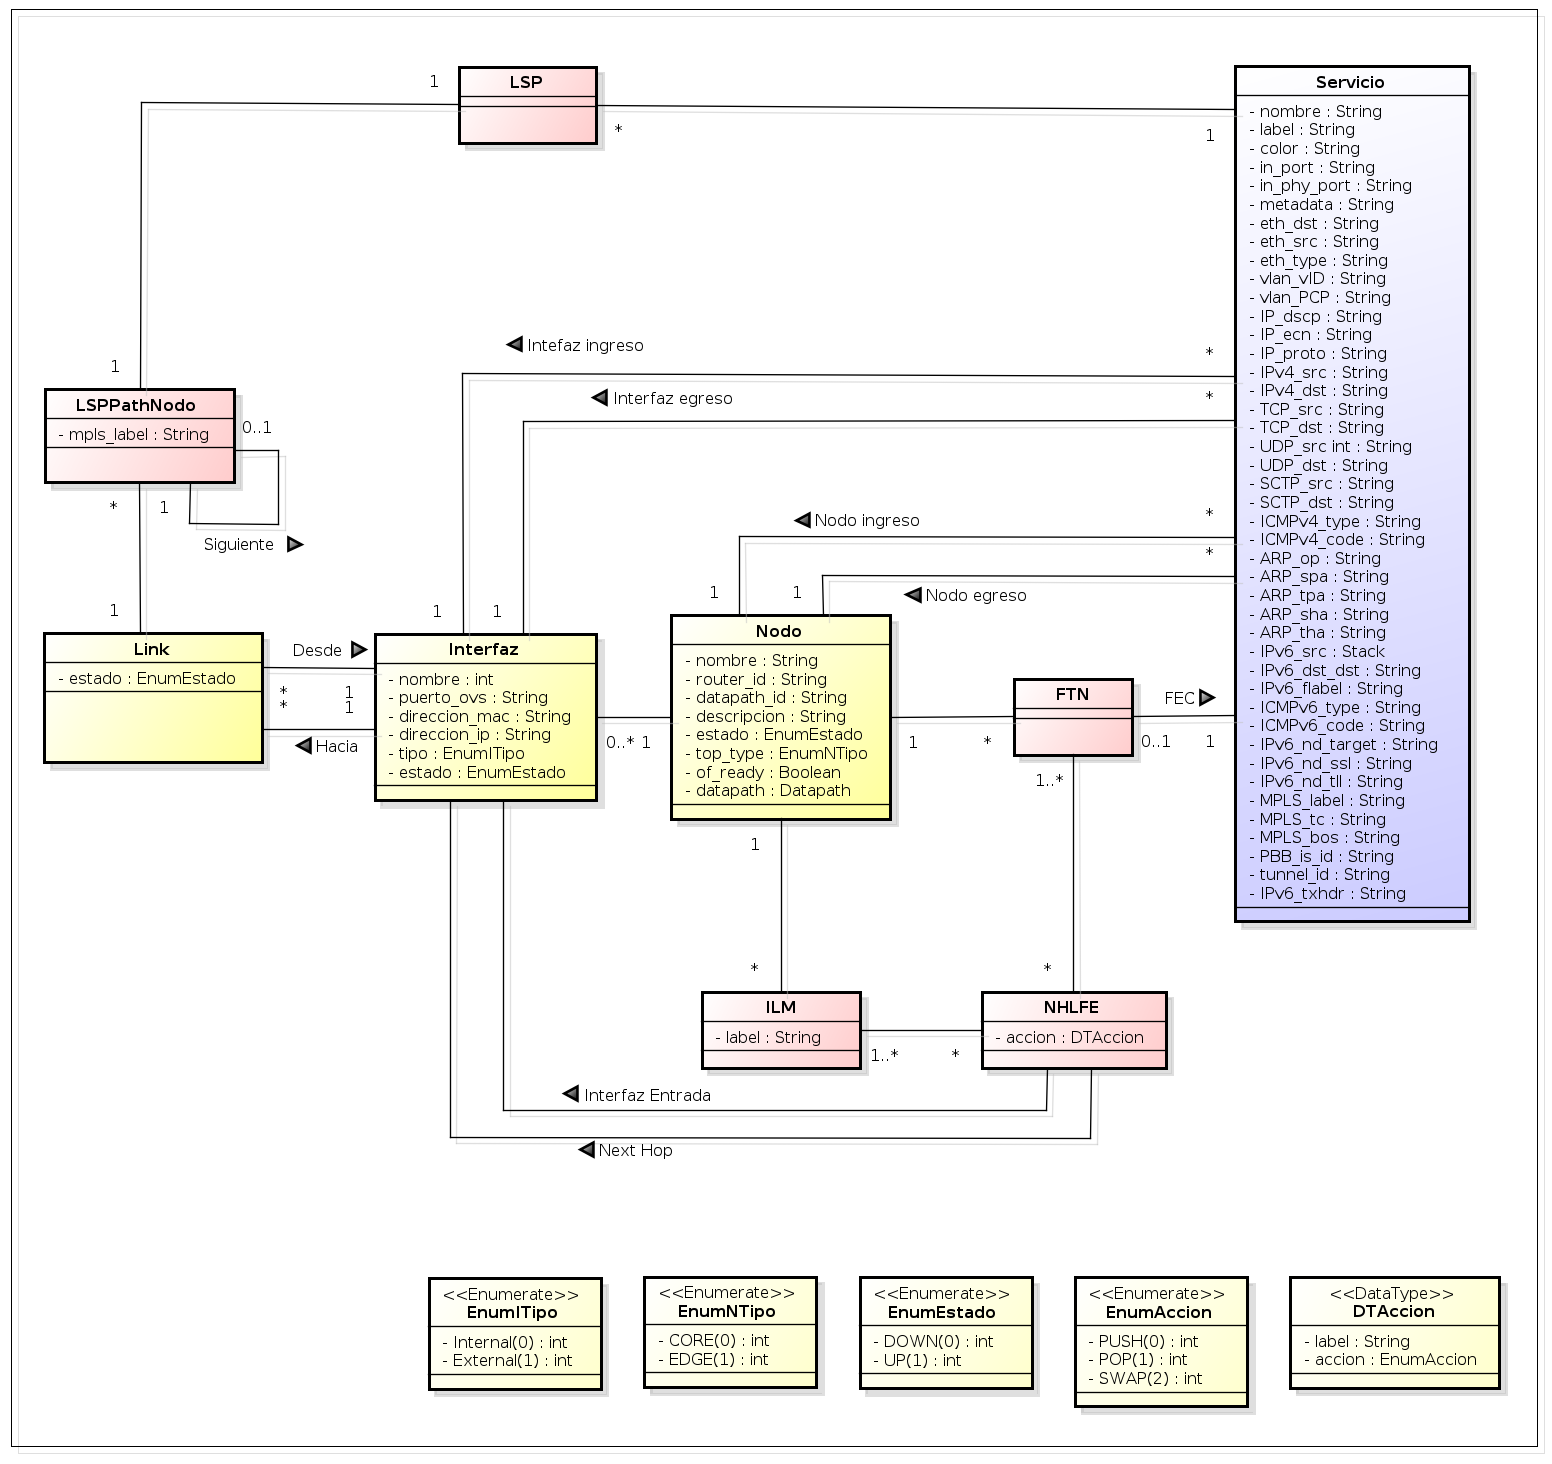
\includegraphics[width=1\textwidth]{DiagramaClases}
\caption[Modelo de datos]{Modelo de datos}
\label{fig:ModeloDeDatos}
\end{figure}

En un mulrigrafo dirigido se tienen nodos y aristas con sentido. Cada nodo de la red puede ser representado por un nodo del grafo y cada enlace entre un par de nodos con dos aristas (una arista para cada sentido del enlace).

En el modelo se tiene adem\'as el concepto de Interfaz de dispositivo. Este concepto re-define la noción de adyacencia entre dos nodos en el grafo de la siguiente forma: existe una arista para un par de nodos si cada uno de ellos est\'a asociado a una instancia de la clase Interfaz y existe una instancia de la clase Link asociada a ambas interfaces mediante las relaciones “Desde” y “Hacia”; indicando adem\'as \'estas el sentido del dicho Link.

Cabe destacar que en el modelo la clase Nodo representa solamente dispositivos de capa 3. Esto quiere decir que dispositivos de capa 2 como switches no son contemplados. Sin embargo no se asume que el nodo est\'e f\'isicamente implementado por RAU-Switch, con lo que se permite modelar nodos implementados en base a otro tipo de dispositivos.

Por otro lado en rosado se destacan las clases utilizadas para representar los principales conceptos de \textbf{MPLS} como las tablas FTN, ILM, NHLFE y el concepto de LSP. Si bien esta \'ultima clase no tiene atributos asociados en esta versi\'on del modelo de datos, eventualmente tiene sentido en un futuro que se puedan asociar atributos del camino como el m\'aximo ancho de banda disponible y algunas otras propiedades orientadas a funcionalidades de QoS.

Finalmente en azul se destaca el concepto Servicio con el cual se busca representar un servicio de red privada virtual. En particular cada instancia de Servicio representa una red privada punto a punto entre dos nodos en el prototipo; por ello esta clase tiene asociados los atributos nodo de ingreso y nodo de egreso. Adem\'as se asume que por cada nodo de borde se tiene a lo sumo una \'unica red privada conectada directamente a cada interfaz. Por ello un servicio queda determinado por los pares <nodo, interfaz> origen y <nodo, interfaz> destino. Luego una red privada multipunto puede construirse definiendo servicios punto a punto para cada par de nodos involucrados.

Esta clase también tiene asociados atributos con los cuales se implementa clasificaci\'on de tr\'afico; m\'as adelante en este cap\'itulo se detallan este y otros aspectos asociados a la implementaci\'on de esta clase.

Teniendo en cuenta los requerimientos mencionados, y el modelado de la realidad presentado, se procede a identificar los casos de uso. 

\section[Casos de uso]{Casos de uso}
\label{section5.3}

La lista de casos de uso presentada a continuaci\'on se corresponde con un conjunto de funcionalidades b\'asicas, que permiten explorar el potencial del enfoque SDN aplicado a la implementaci\'on del prototipo para la RAU2.

\begin{itemize}
\item \textbf{CU1. Listar Servicios}: Devuelve un listado con los servicios existentes en el sistema, mostrando para cada uno la informaci\'on b\'asica asociada.

\item \textbf{CU2. Seleccionar Servicio}: Selecciona un Servicio de un listado(CU2. Listar servicios).

\item \textbf{CU3. Ver Servicio}: Devuelve la informaci\'on asociada al Servicio.

\item \textbf{CU4. Modificar Servicio}: Modifica una instancia de Servicio, actualizando los atributos seleccionados por el usuario con los valores ingresados.
 								
\item \textbf{CU5. Eliminar Servicio}: Elimina un Servicio existente en el Sistema.

\item \textbf{CU6. Agregar Servicio}: Crea un nuevo Servicio de red privada en el Sistema, con la informaci\'on de nodos y sus respectivas interfaces a las que las subredes est\'an directamente conectadas con la red del prototipo. Adem\'as solicita para cada servicio los datos utilizados para la clasificaci\'on del tr\'afico asociado. 

\item \textbf{CU7. Ver Topolog\'ia}: Muestra la topolog\'ia de red mediante una representaci\'on gr\'afica.

\item \textbf{CU.8 Filtrar LSPs}: Superpone en la representaci\'on gr\'afica de la red (CU7.Ver Topolog\'ia) un conjunto de LSPs seleccionados.

\item \textbf{CU9. Seleccionar Nodo}: Selecciona un nodo de una lista de Nodos (CU7. Ver Topolog\'ia).

\item \textbf{CU10. Ver informaci\'on b\'asica Nodo}: Despliega la informaci\'on asociada al nodo seleccionado de la topolog\'ia (CU9. Seleccionar Nodo).

\item \textbf{CU11. Ver tabla de Flujos Nodo}: Muestra la informaci\'on de la tabla de flujos OpenFlow asociada al nodo seleccionado (CU9. Seleccionar Nodo).

\item \textbf{CU12. Ver tablas MPLS}: Muestra la informaci\'on asociada a las tablas FTN, ILM y NHLFE asociadas al nodo seleccionado (CU9. Seleccionar Nodo).

\item \textbf{CU13. Editar Informaci\'on extra Nodo}: Permite ingresar informaci\'on adicional sobre un Nodo como el Nombre y el tipo (nodo interno o de borde).

\item \textbf{CU14. Editar Informaci\'on extra Interfaz}: Ingresa informaci\'on adicional sobre la interfaz de un nodo seleccionado (CU9. Seleccionar Nodo), por ejemplo si la interfaz es interna o externa.
\end{itemize}

En la figura \ref{fig:CasosDeUso} se representan las dependencias existentes entre los casos de uso mencionados anteriormente.

\newpage
\begin{figure}[ht!] 
\centering    
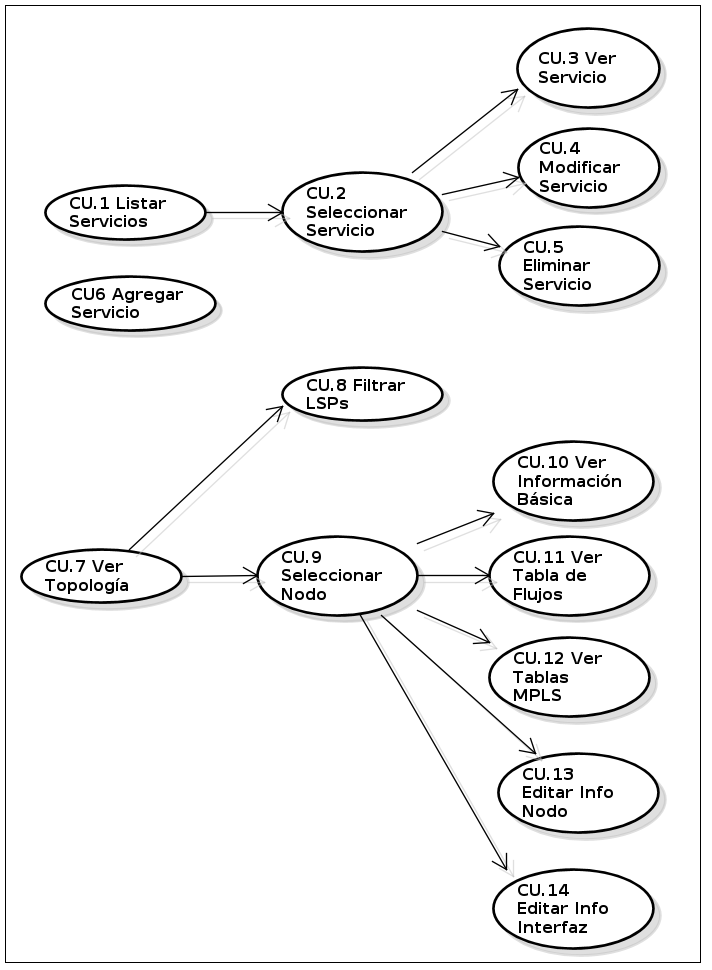
\includegraphics[width=0.7\textwidth]{CasosDeUso}
\caption[Casos de Uso de RAUFlow]{Casos de Uso de RAUFlow}
\label{fig:CasosDeUso}
\end{figure}

En la siguiente secci\'on se presenta la arquitectura de la aplicaci\'on RAUFlow, detallándose las componentes m\'as importantes.

\section[Arquitectura de RauFlow]{Arquitectura de RauFlow}

Como se menciona en el cap\'itulo anterior, RAUFlow es el nombre dado a la aplicaci\'on encargada de implementar el plano de control en el prototipo. Sin embargo como se menciona tambi\'en en dicho cap\'itulo, la o las aplicaciones que se ejecutan en el controlador Ryu interact\'uan con diferentes m\'odulos y componentes como el Administrador SNMP o la base de datos topol\'ogica de Quagga. Por esta raz\'on tiene sentido pensar en RAUFlow como el conjunto de todas estas componentes las cuales interactuando entre ellas implementan efectivamente el plano de control.

Conceptualmente RAUFlow es un conjunto de aplicaciones de control y gestión de red, basada en el enfoque de SDN e implementado utilizando el software de Control Ryu y el protocolo OpenFlow entre otras tecnologías. No es puramente una aplicaci\'on OpenFlow puesto que como se ha mencionado reiteradas veces utiliza un conjunto de componentes y m\'odulos independientes del ambiente del controlador Ryu.

\begin{figure}[h] 
\centering    
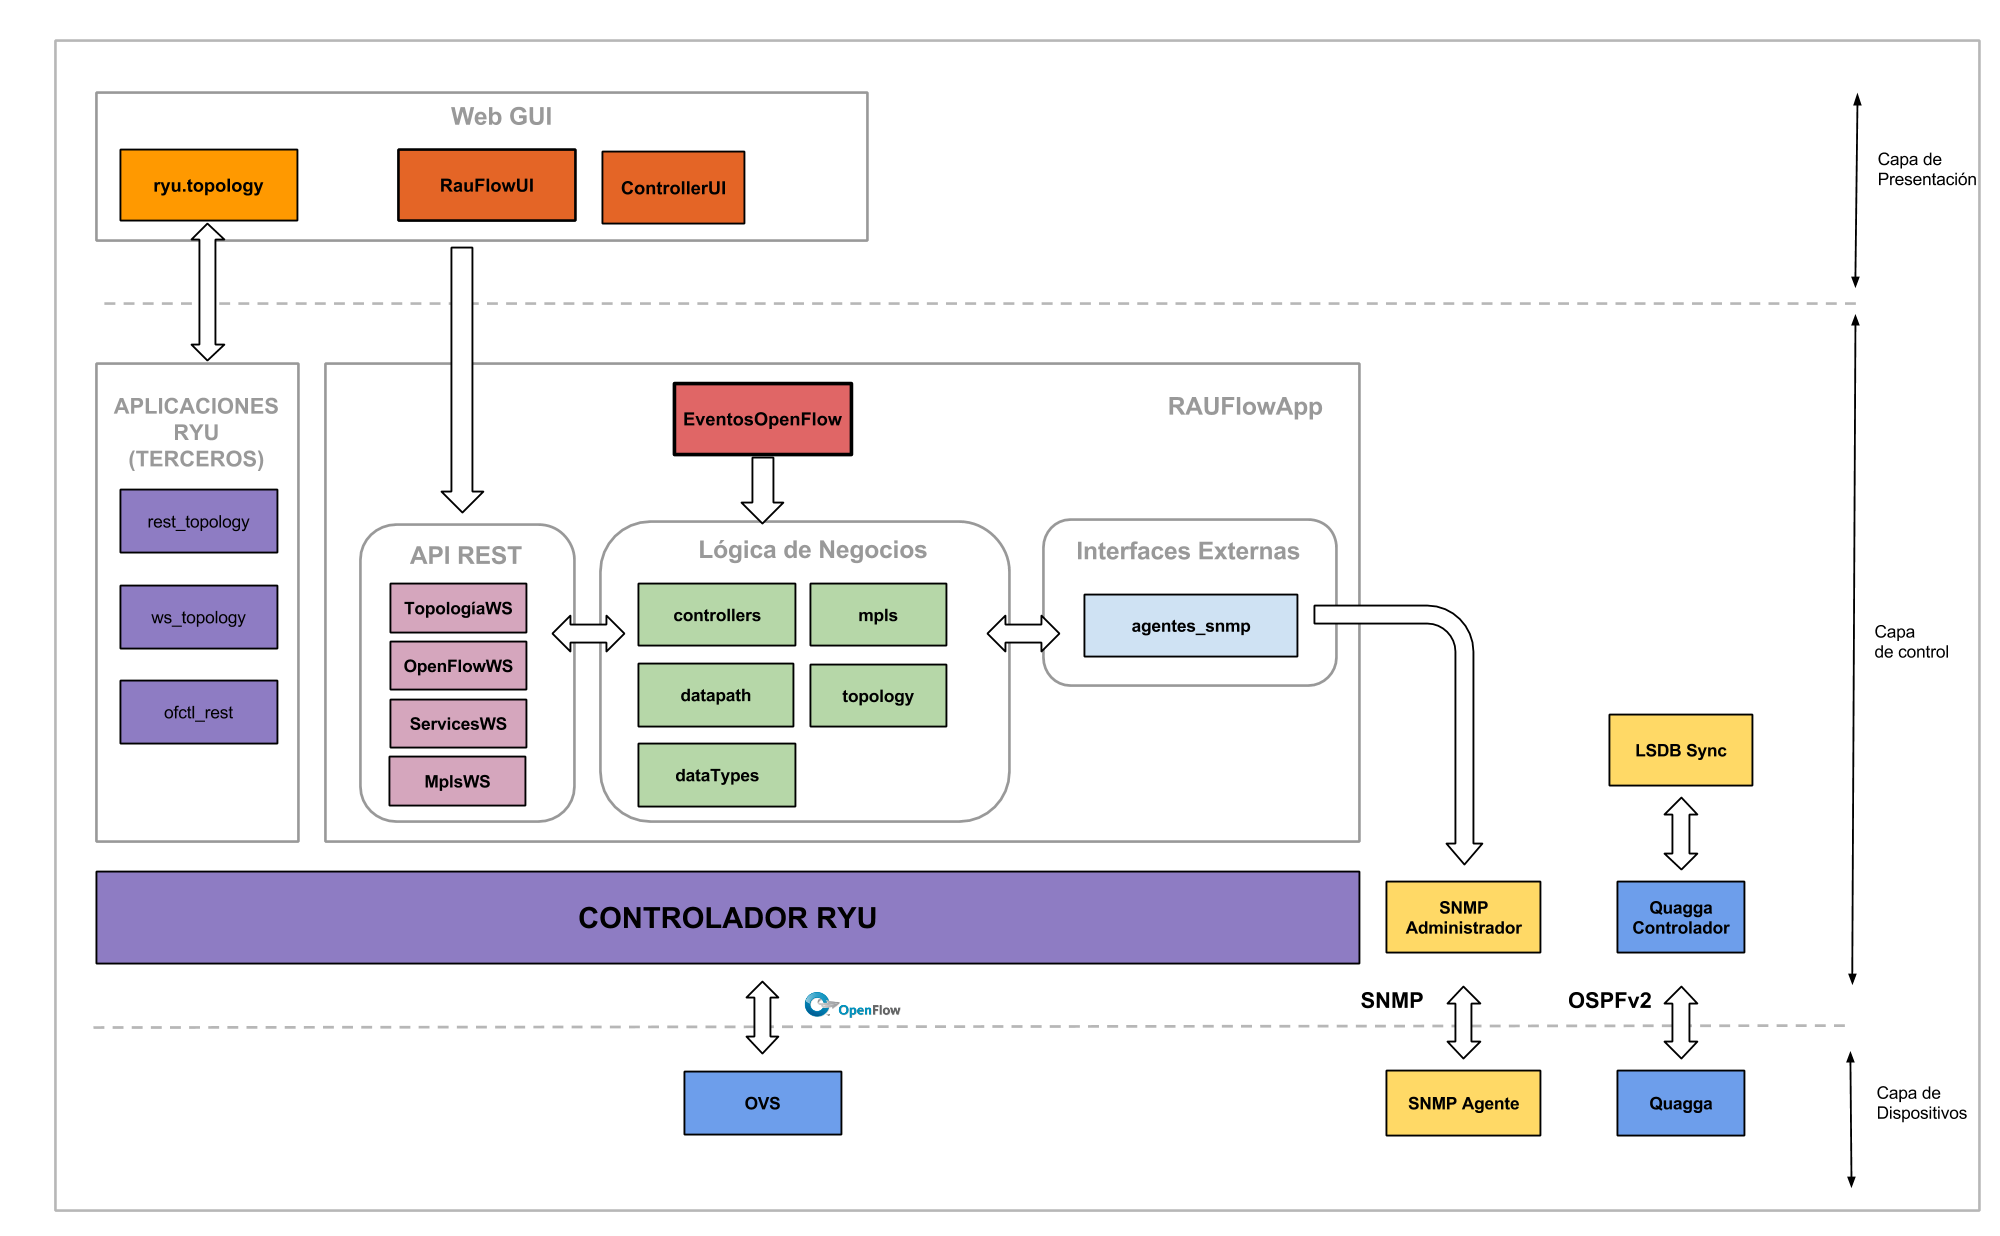
\includegraphics[width=1.0\textwidth]{Disenio_Figure4}
\caption[Arquitectura de RAUFlow]{Arquitectura de RAUFlow}
\label{fig:VistaComponentes2}
\end{figure}

Teniendo en cuenta lo anterior, la arquitectura de la aplicaci\'on (ver figura \ref{fig:VistaComponentes2}), se caracteriza por un diseño en tres capas l\'ogicas: (1) capa de presentaci\'on, (2) capa de control y (3) capa de dispositivos. A continuac\'ion se explica en detalle cada una de estas capas, as\'i como la interacci\'on entre ellas y los principales detalles de los m\'odulos que las componen.

\subsection{Capa de Presentación}
Esta capa est\'a destinada a proveer funcionalidades para el acceso y manipulaci\'on de datos de la aplicaci\'on (estado de la topolog\'ia e informaci\'on asociada a servicios de redes privadas), as\'i como todas las funcionalidades especificadas como requerimientos en la secci\'on 
\ref{section5.1}.

Dentro de la capa de presentaci\'on se destacan: (1) una interfaz gr\'afica identificada en el esquema como RauFlowUI, la cual implementa cada uno de los casos de uso mencionados en la secci\'on \ref{section5.3}, (2) ControladorUI, componente que implementa los m\'etodos de acceso entre las funcionalidades de RauFlowUI y la capa de control a trav\'es de una API Rest de Servicios en la capa de control y (3) un m\'odulo javascript denominado \textbf{ryu.topology}.

Ryu incluye a modo de documentaci\'on un conjunto de aplicaciones muy sencillas en las que se ejemplifica el uso de las principales funcionalidades del protocolo OpenFlow. Entre estas aplicaciones se encuentra \textbf{gui\_topology}, la cual brinda una representaci\'on gr\'afica b\'asica de las componentes topol\'ogicas en una red OpenFlow (switches, puertos y links). Esta aplicaci\'on a su vez se basa en tres aplicaciones Ryu de la capa de control (m\'as adelante se detalla el funcionamiento de ellas cuando se explique la capa de control), una pagina web desarrollada puramente sobre HTML y un m\'odulo de javascript encargado de la manipulaci\'on de informaci\'on entre las aplicaciones Ryu y esta p\'agina mediante websockets (este m\'odulo recibe el nombre de \textbf{ryu.topology}).

En RAUFlow se combinan las componentes de la aplicaci\'on \textbf{gui\_topology} como el m\'odulo javascript \textbf{ryu.topology} y las tres aplicaciones Ryu con el resto de las componentes de la aplicaci\'on con el objetivo de mejorar la interfaz gr\'afica RAUFlowUI, brindando una representaci\'on gr\'afica del estado topol\'ogico de la red reutilizando las herramientas existentes.
 
\subsection{Capa de Control}

La capa de control est\'a conformada por cuatro componentes: el software de control Ryu con su respectivo conjunto de aplicaciones SDN, el m\'odulo LSDBSync, el m\'odulo Administrador SNMP y la instancia de Quagga ejecutada en el Controlador.

\subsubsection{Aplicaciones RYU (Terceros)}
En RAUFlow se ejecuta un conjunto de tres aplicaciones con el objetivo de facilitar la representaci\'on gr\'afica del estado de la topolog\'ia, a partir de las funcionalidades de la aplicación \textbf{gui\_topology}, anteriormente mencionada. 

Las tres aplicaciones utilizadas son:
(1) rest\_topology, (2) ws\_topology y (3) ofctl\_rest. Las funcionalidades de cada una de estas aplicaciones son las siguientes:

\begin{enumerate}
\item rest\_topology: Implementa una API REST de servicios para el acceso a informaci\'on topol\'ogica de switches OpenFlow y links existentes entre ellos. Esta API es utilizada por \textbf{ryu.topology} para construir la representaci\'on gr\'afica de la red.

\item ws\_topology: Mantiene en memoria informaci\'on de cada switch de la capa de dispositivos registrado con el controlador. A su vez gestiona eventos OpenFlow generados cuando un switch se reporta o deja de reportarse, cuando cambia el estado de un puerto, cuando llega un paquete, entre otros eventos del protocolo.

\item ofctl\_rest: Mediante una API REST de servicios expone un conjunto de m\'etodos para acceder a informaci\'on del plano de datos OpenFlow (datapath OpenFlow) y as\'i obtener todo tipo de informaci\'on relacionada a un switch en particular. Implementa desde m\'etodos para obtener la tabla de flujos de un dispositivo, estadísticas agregadas por flujo, puerto, grupo de puertos y colas entre otros. Esta aplicaci\'on es utilizada por la p\'agina web original de \textbf{gui\_topology} y por RAUFlowUI en la arquitectura de RAUFlow para el acceso a informaci\'on estad\'istica de la tabla de flujos de un switch.

\end{enumerate}

Por otro lado se ejecuta sobre el controlador una cuarta aplicaci\'on Ryu. A continuaci\'on se detalla su estructura y funcionamiento.

\begin{subsubsection}{RAUFlowApp}
Dentro de las aplicaciones Ryu, RauFlowApp es realmente la encargada de implementar el plano de control  del prototipo. Esto quiere decir, guardar informaci\'on de la realidad, servicios de redes privadas creados, guardar el estado de la topolog\'ia, implementar funcionalidades de QoS, ruteo din\'amico etc. Vale la pena aclarar, que a diferencia de las tres aplicaciones anteriores, las cuales fueron desarrolladas por el equipo detrás del software Ryu, esta aplicaci\'on es completamente diseñada e implementada en el marco de este proyecto.

En relaci\'on al diseño de esta aplicaci\'on, como puede apreciarse en la figura \ref{fig:VistaComponentes2} responde a una organización modular, en la cual se destacan cuatro componentes principalmente: (1) EventosOpenFlow (2) L\'ogica de Negocios, (3) API REST de Servicios y (4) Interfaces Externas. El funcionamiento de cada uno de ellos es el siguiente:
  
\begin{enumerate}

\item EventosOpenFlow\\
EventosOpenFlow es una aplicaci\'on Ryu con el esquema b\'asico de este tipo de programas (las aplicaciones Ryu tienen un esquema particular). Se encarga de proveer m\'etodos para los principales eventos del protocolo OpenFlow; por ejemplo cuando un switch se reporta con el controlador por primera vez o deja de reportarse, cuando el controlador recibe un paquete (Packet IN), cuando se produce un cambio en la topolog\'ia como por ejemplo un puerto en un dispositivo que deja de funcionar, entre otros.

El modelado de la realidad, la implementaci\'on de funcionalidades de acceso a la capa de dispositivos, estructuras de datos almacenadas en memoria, así como los algoritmos de ruteo y distribución de etiquetas son implementados en la componente Lógica de Negocios. De esta forma se desacoplan las responsabilidades, mejorando la claridad y transparencia en el diseño de la aplicaci\'on. No obstante esta aplicación es la responsable de gestionar el ciclo de vida de los diferentes objetos asociados a la componente Lógica de Negocios.
  
\item Lógica de Negocios\\
Como se ha mencionado esta componente es responsable del modelado de la realidad y la implementaci\'on de las principales funcionalidades del plano de control de RAUFlow. Se subdivide a su vez en diferentes m\'odulos que agrupan funcionalidades acorde a su naturaleza y responsabilidad. Vale la pena destacar a su vez que cada uno de estos m\'odulos se corresponde en la implementaci\'on realizada con un m\'odulo de Python. A continuaci\'on se explican las responsabilidades de cada uno de ellos:

\begin{itemize}
\item \textbf{controller:} Este m\'odulo agrupa diferentes controladores de objetos. Actualmente contiene un \'unico controlador fachada responsable de mantener el \'unico punto de acceso a la las componentes de la l\'ogica de negocios. Contiene desde la implementaci\'on de funciones para dar de alta Servicios, crear LSPs, obtener el mejor camino entre dos nodos de la red, entre otras.

\item \textbf{topology:} Agrupa las definiciones de objetos utilizados para representar la topolog\'ia como las clases Nodo, Interfaz y Link, así como otros conceptos de la realidad.
 
\item \textbf{mpls:} Contiene las definiciones de los conceptos FTN, ILM, NHLFE, as\'i como los conceptos de servicio de red y LSP (Label Switched Path).

\item \textbf{dataTypes:} Mantiene representaciones reducidas de los principales objetos definidos en todos los m\'odulos de la componente de negocios para el intercambio de datos por ejemplo con la capa de presentaci\'on. 

\item \textbf{datapath:} Agrupa funcionalidades para el acceso al datapath de OpenFlow, como funciones para agregar y eliminar flujos en un switch, u obtener estad\'isticas de una tabla de flujos.
\end{itemize} 

Para acceder a la componente de Lógica de Negocios se tiene una API REST de Servicios.

\item API REST de servicios\\
Esta componente define m\'etodos para el acceso a los datos y funcionalidades de la componente Lógica de Negocios. Es utilizada por la capa de Presentaci\'on para acceder a informaci\'on de la realidad o crear nuevos servicios. A su vez es utilizada por otras componentes de la capa de control como lo es el caso del m\'odulo LSDBSync para enviar informaci\'on actualizada de la topolog\'ia de red al momento de ejecutar RAUFlow por primera vez y luego cuando la topolog\'ia cambia. 

Se subdivide en varios m\'odulos respondiendo al criterio utilizado para el dise\~no modular de la anterior componente. 

\item Interfaces Externas\\
Cuando se enciende RAUFlow y se recibe por primera vez la informaci\'on topológica, o cuando la topolog\'ia cambia y se produce una actualizaci\'on, es necesario obtener informaci\'on adicional sobre cada dispositivo (hecho ya mencionado en reiteradas ocasiones). Para esto la aplicaci\'on utiliza la componente denominada Interfaces Externas. Esta componente funciona como punto de conexi\'on entre la componente L\'ogica de Negocios y otras componentes externas a la aplicaci\'on RAUFlowApp. Un ejemplo de una componente externa es el m\'odulo Administrador SNMP, encargado de obtener la informaci\'on extra en el proceso de actualizaci\'on topol\'ogica mencionado, utilizando el Agente SNMP instalado en cada dispositivo RAU-Switch del prototipo.

Dentro de esta componente, actualmente existe un solo mo\'dulo denominado \textbf{agentes\_snmp}. Este m\'odulo es el encargado de la ya mencionada comunicaci\'on con el m\'odulo Administrador SNMP.

\end{enumerate}

\end{subsubsection}

\subsubsection{Administrador SNMP}
El funcionamiento de este m\'odulo se ha explicado anteriormente en el cap\'itulo 4.

\subsubsection{LSDB Sync}
Como se muestra en el diagrama de arquitectura, este m\'odulo interact\'ua con la instancia de Quagga instalada en el controlador en dos formas distintas. Por un lado advierte cuando la topolog\'ia cambia observando los mensajes que se env\'ian a través del protocolo OSPF en la red, y por otro lado accede, procesa y env\'ia la informaci\'on de la base de datos topol\'ogica LSDB local a la aplicaci\'on RAUFlowApp a trav\'es de un web service de la API Rest implementada en esta aplicaci\'on.
 
\subsection{Capa de Dispositivos}
En la capa de dispositivos se muestran las diferentes componentes de RAU-Switch que interactúan con la capa de control, indicando para cada una de ellas el protocolo de comunicaci\'on utilizado.

Por un lado se tiene la herramienta Open vSwitch de la cual tanto su rol en la implementaci\'on del prototipo, como su funcionamiento ya se ha explicado anteriormente. Vale la pena mencionar simplemente, que las \'unicas componentes de la capa de control de RAUFlow que interact\'uan con la misma, adem\'as de las tres aplicaciones que vienen con Ryu, son la aplicaci\'on EventosOpenFlow y el m\'odulo datapath.

Tambi\'en forma parte de la capa de dispositivos, el agente SNMP consultado por el Administrador SNMP en la capa de control mediante el protocolo SNMP.

Finalmente se tiene la instancia de Quagga, la cual a través del intercambio de mensajes del protocolo OSPF con las restantes instancias de Quagga en cada dispositivo RAU-Switch, construyen la base de datos topol\'ogica en el controlador.

Una vez presentada y explicada en detalle la arquitectura de RAUFlow, el lector est\'a en condiciones de abordar la siguiente secci\'on, en la que se abordan detalles relacionados a la implementaci\'on.

\section[Implementaci\'on]{Implementaci\'on}

En esta secci\'on se presentan los aspectos m\'as importantes relacionados a la implementaci\'on de RauFlow. Entre ellos se destacan la estrategia utilizada para implementar clasificaci\'on de tr\'afico,  la implementaci\'on de la clase servicio, la implementaci\'on de los algoritmos de ruteo y distribución de etiquetas, entre otros.

\subsection{Clasificación de tr\'afico}
En la arquitectura MPLS, tradicionalmente se utiliza el concepto de FEC (fordwarding equivalence class) para distinguir a un conjunto de paquetes a ser tratados en forma similar (por ejemplo para aplicar t\'ecnicas de QoS). Este concepto se define localmente a un dispositivo, determinando la forma en que un conjunto de paquetes son tratados solamente en el mismo.

En RAUFlow se aprovecha la visi\'on global del plano de control SDN para definir una noci\'on de FEC global en una topolog\'ia de red. En esta redefinici\'on se clasifica tr\'afico solamente en el nodo de ingreso a la red del prototipo, determinándose all\'i el camino a seguir por un paquete hasta el nodo de egreso mediante el resultado obtenido en la ejecuci\'on del algoritmo de ruteo. 

Por otro lado se define un mapeo entre servicios de VPN y etiquetas MPLS, permitiendo identificar el tr\'afico asociado a un servicio particular en cualquier nodo de la red. Luego a partir del valor de esta etiqueta se puede realizar un procesamiento diferencial en nodos intermedios de un LSP.

En relaci\'on a como se implementa clasificaci\'on de tr\'afico, en el prototipo se utilizan las tablas de flujos de Open vSwitch en conjunto con los campos del cabezal OpenFlow (matching fields) para la definici\'on de flujos. Con los matching fields de OpenFlow se define la regla de un flujo (recordar figura \ref{fig:OpenFlowArch2}) distinguiendo de este modo entre diferentes clases de tr\'afico para un procesamiento diferencial.

Dentro del cabezal OpenFlow, existen campos para la definici\'on de las reglas de un flujo, campos para la definici\'on de la acci\'on de un flujo y campos que pueden ser utilizados para la definici\'on de ambas componentes. Esta lista de campos var\'ia con la versi\'on del protocolo OpenFlow y en el contexto del prototipo est\'a acotada a su vez por la implementaci\'on de Open vSwitch. En el ap\'endice \ref{appendix3} se muestra  la lista entera de atributos que contiene el cabezal OpenFlow para la versi\'on 1.3.1 y de \'estos la lista de atributos que son soportados por Open vSwitch y que pueden ser utilizados para la definici\'on de reglas y acciones. Ambas listas fueron construidas experimentalmente trabajando con las herramientas Open vSwitch y Ryu.

En el prototipo, el concepto de clasificaci\'on de tr\'afico est\'a estrictamente ligado al concepto de servicio de red privada. En la siguiente secci\'on se explica en detalle la implementaci\'on de este concepto.
 
\subsection{Implementación de Servicio}

La clase Servicio implementa el concepto de servicios de red privada virtual. Como se menciona anteriormente un servicio define una clase de tr\'afico; por tanto adem\'as de la informaci\'on b\'asica que define a un servicio se tienen asociados tambi\'en todos los campos utilizados para implementar clasificaci\'on de tr\'afico (matching fields de OpenFlow).

En el prototipo se asume que por cada nodo de borde  se tiene una \'unica red privada directamente conectada a cada interfaz externa. Esto permite definir un servicio a partir de la clase de tr\'afico definida y los pares nodo-interfaz origen y nodo-interfaz destino.

Por otro lado se podr\'ia refinar la definici\'on de servicio agregando m\'as dimensiones; una dimensi\'on bastante \'util podr\'ia ser por ejemplo el tiempo, donde se podr\'ia por ejemplo definir un servicio de red privada para un rango horario determinado.

De igual forma se pueden incorporar m\'as dimensiones orientado a brindar una mayor flexibilidad en la definici\'on de servicios, de cara a lo que podr\'ian ser diferentes requerimientos de la RAU2. 

De todos modos teniendo en cuenta el alcance del proyecto se decide dejar estas dimensiones extras como una posible l\'inea de trabajo a futuro.

De esta forma la clase servicio queda determinada de la siguiente forma:

\begin{python}
class Service (object):

		# Atributos generales
		ID 				    # str (uuid.uuid4()) ID unico  
		name 				# Nombre del servicio para 
							
		lsps				# Lista de LSPs para el servicio
		
		ingress_node		# Nodo de ingreso del servicio
		egress_node 		# Nodo de egreso del servicio			
		ingress_interface 	# Interfaz de ingreso en el nodo 
							# de ingreso		
		egress_interface 	# Interfaz de egreso en el nodo 
							# de ingreso 
        
		# Campos del cabezal OFv1.3 
		in_port			# Switch input port. 
		metadata 		# Metadata passed between tables. 
		eth_dst 		# Ethernet destination address.
		eth_src 		# Ethernet source address. 
		eth_type 		# Ethernet frame type. 
		vlan_vID 		# VLAN id. 
		vlan_PCP		# VLAN priority. 
		IP_dscp 		# IP DSCP (6 bits in ToS field). 
		IP_ecn  		# IP ECN (2 bits in ToS field). 
		IP_proto		# IP protocol. 
		IPv4_src 		# IPv4 source address. 
		IPv4_dst 		# IPv4 destination address. 
		TCP_src 		# TCP source port. 
		TCP_dst 		# TCP destination port. 
		UDP_src 		# UDP source port. 
		UDP_dst 		# UDP destination port. 
		SCTP_src 		# SCTP source port. 
		SCTP_dst 		# SCTP destination port. 
		ICMPv4_type 	# ICMP type. 
		ICMPv4_code 	# ICMP code. 
		IPv6_src 		# IPv6 source address. 
		IPv6_dst 		# IPv6 destination address. 
		ICMPv6_type 	# ICMPv6 type. 
		ICMPv6_code 	# ICMPv6 code. 
		MPLS_label 		# MPLS label. 
		MPLS_tc 		# MPLS TC. 
		
\end{python}

En RAUFlow, cuando se crea un nuevo servicio se ejecutan los algoritmos de ruteo y distribución de etiquetas para construir al menos un LSP. Luego el mismo es traducido a flujos OpenFlow que luego son instalados en cada uno de los nodos en el mismo. 

En la siguiente secci\'on se detalla el algoritmo de ruteo utilizado en RAUFlow.

\subsection{Algoritmo de ruteo}
El algoritmo de ruteo implementado parte de un algoritmo Shortest Path First (SPF) centralizado para el c\'alculo del mejor camino entre un par de nodos en la topolog\'ia. Luego incorporando restricciones al mismo es posible llegar a un Constrained Shortest Path First (CSPF) con el cual se podr\'ia implementar funcionalidades de QoS.

En el desarrollo de este proyecto, por razones de tiempo solo fu\'e posible la implementaci\'on del algor\'iitmo SPF centralizado. De esta forma la implementaci\'on de un algoritmo de ruteo CSPF se identifica como una posible l\'inea de trabajo a futuro. A continuaci\'on se explica la implementaci\'on del algoritmo SPF. 

\subsubsection{Shortest Path First}
El algoritmo SPF centralizado est\'a basado en el algoritmo Dijkstra. Este algoritmo permite calcular en forma eficiente el mejor camino entre un par de nodos en un grafo ponderado sin costos negativos.

Puesto que en este trabajo se representa a una topolog\'ia de red mediante un multigrafo dirigido, es necesario o bien extender el algoritmo Dijkstra a esta representaci\'on o bien cambiar de representaci\'on. Como los multigrafos dirigidos ofrecen un modelado de la realidad intuitivo y directo, se opta por la alternativa de extender el algoritmo Dijkstra. Cabe destacar la existencia de trabajos previos en el desarrollo de una posible extensi\'on a este algoritmo para multigrafos; en este trabajo se sigue la propuesta de \cite{biswas2013generalization}.

En \ref{fig:algoSPF1} se muestra el pseudo-c\'odigo del algoritmo SPF centralizado para multigrafos dirigidos obtenido a partir de la extensi\'on del algoritmo Dijkstra. Este recibe como par\'ametros la topolog\'ia de red (G) y el par de nodos inicio y fin para el cual se quiere calcular el mejor camino posible. Las operaciones \textit{ObtenerNodosMenorCostoLink} y \textit{ObtenerNodoAdyacenteMenorCosto} son funciones auxiliares que se explican a continuación:

\begin{itemize}
\item ObtenerNodosMenorCostoLink (w, v): Permite obtener el link <w, v> de menor costo asociado en la topolog\'ia entre los nodos w y v. Notar que para un par de nodos w, v pueden existir m\'ultiples enlaces que los conecten, eventualmente con costos diferentes. 

\item ObtenerNodoAdyacenteMenorCosto ($G\setminus S$, D): Devuelve el nodo en $G\setminus S$ para el cual el costo de ir desde el nodo inicio a este es m\'inimo en la lista de costos D.
\end{itemize}

\newpage
\begin{figure}[ht!] 
\begin{algorithm}[H]
 \SetKwFunction{CaminoMasCortoMultigrafo}{CaminoMasCortoMultigrafo} 
 \SetKwProg{myalg}{Function}{}{}
 \myalg{\CaminoMasCortoMultigrafo(G, inicio, fin){}}{\Comment{Obtiene el mejor camino en G entre los  					nodos inicio y fin, utilizando como m\'etrica el costos asociado a cada adyacencia}\\
  \textbf{Pre-condiciones:} inicio $\in$ G y fin $\in$ G\\
  \vspace{0.3cm}
  
  camino[] $\gets \lbrace\rbrace$\\														
 
  D,P $\gets$ MultiDijkstra(G, inicio, fin) \Comment{Utiliza algoritmo Dijkstra para obtener el mejor 
  													camino }\\
  i $\gets$ fin \Comment{Arma el camino en función de la lista de predecesores}\\
  \While{i $<>$ inicio}{
  	l $\gets$ P[i]\\
  	camino $\gets$ camino  $\cup$ l\\
  	i $\gets$ l.origen\\
  } 
  
  camino.Reverse()\Comment{Hay que invertir el orden del camino}\\
  
 \Return{camino}  
 }
\end{algorithm}
\caption[Algoritmo de ruteo centralizado sin restricciones (SPF)]{Algoritmo de ruteo centralizado sin restricciones (SPF)}
\label{fig:algoSPF1}
\end{figure}

\newpage
\begin{figure}[ht!] 
\begin{algorithm}[H]
 \SetKwFunction{MultiDijkstra}{MultiDijkstra} 
 \SetKwProg{myalg}{Function}{}{}
 \myalg{\MultiDijkstra(G, inicio, fin){}}{\Comment{Extensión de algoritmo Dijkstra para c\'alculo de
  		mejores caminos en un multigrafo dirigido ponderado}\\

	\vspace{0.5cm}
	
 	D $\gets \lbrace\rbrace$   \Comment{Distancias finales}\\
    P $\gets \lbrace\rbrace$  \Comment{Lista de links predecesores <nodo\_origen, nodo\_destino>}\\
    S $\gets \lbrace\rbrace$ \Comment{Lista de nodos procesados}\\
    GmenosS $\gets$ G \Comment{Inicializa G $\setminus$ S como G}\\
    
    \vspace{0.2cm}
        
    S $\gets$ S $\cup$ inicio\Comment{El algoritmo empieza con nodo inicio}\\
    GmenosS $\gets$ GmenosS $- \lbrace inicio \rbrace$\\
    
    \ForEach{i in G}{
    	\uIf{i in G[inicio]}{\Comment{Si los nodos son adyacentes actualiza el costo en D y el link 	
    								predecesor}
    		l $\gets$ ObtenerNodosMenorCostoLink(inicio, i)\Comment{Obtiene el link de 
    																	menor costo entre los nodos}\\
    		D[i] $\gets$ l.costo\\
    		P[i] $\gets$ l\\	
 		}
 		\Else{
 			D[i] $\gets$ -1\\
            P[i] $\gets$ Null \\ 		
 		}
    }
    
    \vspace{0.2cm}

    \For{i in (1 \dots $\vert G \vert$)}{
    	w = ObtenerNodoAdyacenteMenorCosto(GmenosS, D)\Comment{Obtiene el nodo adyacente de 	
    																		menor costo}\\
    	S $\gets$ S $\cup$ w\\
    	GmenosS $\gets$ GmenosS $- \lbrace w \rbrace$\\
    	\Comment{Actualiza la lista de costos y predecesores para todos los nodos en $G\setminus S$}\\
    	\ForEach{v in GmenosS}{
			l $\gets$ ObtenerNodosMenorCostoLink(w, v)\\
			\If{ l <> Null AND (D[v] = -1 OR D[w] + l.costo < D[v])}{
				D[v] $\gets$ D[w] + l.costo\\
                P[v] $\gets$ l\\
			}    	
    	}
    }
  	  
 \Return{(D, P)} 
 \vspace{1cm} 
 }
 
\end{algorithm}
\caption[]{SPF Centralizado continuaci\'on}
\end{figure}

\newpage
\subsection{Algoritmo de distribución de etiquetas}
\label{section5.5.4}

MPLS utiliza etiquetas para: (a) distinguir el tr\'afico de una VPN particular y (b) encaminar tr\'afico en la red (reenvío en base a etiquetas). De esta forma se tienen dos niveles de etiquetas usualmente denominadas inner label (para marcar el tr\'afico) y outer label (para encaminar tr\'afico - LSP).

Para la distribución de etiquetas (inner y outer label) existen diferentes protocolos entre los cuales puede destacarse el protocolo LDP (Label Distribution Protocol)~\citep{LDPRFC}. Este protocolo representa un buen modelo a seguir para el algoritmo de distribución de etiquetas, pero est\'a definido en base a la visión topol\'ogica local de un nodo, mientras que en RAUFlow es necesario definir un algor\'itmo basado en una visi\'on topol\'ogica global. Por ello es necesario implementar un algoritmo de distribución de etiquetas diferente.

A continuaci\'on se explican los algoritmos utilizados para la distribución de etiquetas de ambos niveles.

\subsubsection{Etiquetas internas (Inner Labels)}
Mapear etiquetas MPLS a servicios de VPN para posteriormente poder identificar el tr\'afico asociado dentro del prototipo es una tarea bastante simple. Una soluci\'on posible es asignar secuencialmente etiquetas dentro de un espacio de etiquetas disponible. Esta estrategia es simple y permite crear en el sistema tantos servicios como etiquetas disponibles. Puesto que una etiqueta MPLS se representa mediante 20bits $= 2^{20}$ posibles valores, descontando los  valores reservados por el protocolo se pueden crear m\'as que suficientes servicios utilizando esta estrategia.

No obstante, si bien esta estrategia es suficiente para la asignación de la etiqueta interna m\'as adelante se ver\'a que es necesario modificarla ligeramente para soportar ciertos casos de uso en el prototipo.

\subsubsection{Etiquetas externas (Outer Label)}
Asignar etiquetas a un camino MPLS es un problema m\'as complejo. Aprovechando la visión global de la red puede redefinirse el algoritmo de distribución de etiquetas LDP de varias formas. Algunas de ellas pueden ser:

\begin{enumerate}
\item Asignar secuencialmente etiquetas a cada salto en un camino utilizando un espacio de etiquetas global para el LSP. De esta forma no existen dos LSPs en el sistema con etiquetas en com\'un. Esta solución tiene como ventajas su simplicidad y bajo costo en el c\'omputo del algoritmo. Por otro lado tiene como desventaja que consume el espacio de etiquetas disponibles m\'as r\'apido (hay que considerar la escala del prototipo).

\item Asignar secuencialmente etiquetas a cada salto en un camino utilizando un espacio de etiquetas local a cada nodo y descartando para cada interfaz etiquetas ya utilizadas por otros LSPs. Esta estrategia tiene como ventaja que es m\'as austera en el consumo de etiquetas y no existen dos LSPs con iguales etiquetas para una misma interfaz de entrada en un mismo nodo.
\end{enumerate}

N\'otese en relación a la segunda alternativa, que debido a la forma en que se distribuyen etiquetas puede determinarse en un nodo a que servicio corresponde un paquete bas\'andose solamente en la etiqueta externa y la interfaz por la que entra. Esto permite prescindir de la etiqueta interna para determinar lo que en un esquema tradicional de MPLS se denomina FEC y aplicar diferentes pol\'iticas de ingenier\'ia de tr\'afico. Esto a su vez repercute en un aumento del MTU del paquete.

En RauFlow se implementa la segunda alternativa mencionada. En \ref{fig:AlgoritmoDE1} se muestra el pseudoc\'odigo de una posible implementaci\'on de dicho algor\'itmo:

\begin{figure}[ht!]
\begin{algorithm}[H]

 \SetKwFunction{obtenerEtiquetasLSP}{obtenerEtiquetasLSP} 
 \SetKwFunction{obtenerEtiquetaParaInterfaz}{obtenerEtiquetaParaInterfaz}
 \SetKwProg{myalg}{Function}{}{}
 \myalg{\obtenerEtiquetasLSP(path){}}{ \Comment{Recibe una camino en la topolog\'ia representado como 	
 												una lista ordenada de links y devuelve una lista 	
 												ordenada de etiquetas donde cada etiqueta se
 												corresponde a un link}\\
 	
 	\vspace{0.5cm}
 												
    MPLS\_LABEL\_SPACE\_MIN $\gets 10$\\
 	mplsPath[] $\gets \lbrace\rbrace$\\
 	labelBase $\gets$ Null\\
 
	\uIf{len(path) = 1}{
    	$mplsPath \gets mplsPath \cup \{Null\}$ \Comment{Si el camino es de largo 1, no tiene 
    													etiquetas porque primer nodo hace PHP}
 	}
 	\Else{
    	labelBase $\gets$ MPLS\_LABEL\_SPACE\_MIN \Comment{Se asignan etiquetas secuencialmente en el
    														 espacio de etiquetas}
    
   		\ForEach{l in path-1}{
			label $\gets$ \obtenerEtiquetaParaInterfaz(l, labelBase) \Comment{Obtiene una etiqueta 
												libre del espacio de etiquetas local a la interfaz}\\
			
			$mplsPath \gets mplsPath \cup \{label\}$\\
			
			$labelBase \gets labelBase + 1$\\
				
 		}
 		
 		$mplsPath \gets mplsPath \cup \{Null\}$\Comment{Como \'ultimo nodo implementa PHP el 
													\'ultimo link no tiene etiqueta asociada}\\
 	}        
 
 	\Return{mplsPath[]}
 }
\end{algorithm}
\caption[Algoritmo de distribución de etiquetas]{Algoritmo de distribución de etiquetas}
\label{fig:AlgoritmoDE1}
\end{figure}

\newpage
\begin{figure}[ht!]
\begin{algorithm}[H]
\SetKwFunction{obtenerEtiquetaParaInterfaz}{obtenerEtiquetaParaInterfaz}
\SetKwProg{myalg}{Function}{}{}
 \myalg{\obtenerEtiquetaParaInterfaz(link, label){}}{\Comment{Devuelve una etiqueta dentro del espacio de etiquetas global que no este en uso por la interfaz destino en el link. Si no existe etiqueta disponible devuelve Null}\\
 
	\vspace{0.5cm}
	 
	 etiquetas\_usadas $\gets$ link.destino.etiquetas\_usadas\\
	 next\_label $\gets$ label\_base\\
	 label $\gets$ Null\\
	 
	 \While{label == Null AND next\_label $<$ MPLS\_LABEL\_SPACE\_MAX}{
		\uIf{(next\_label in etiquetas\_usadas)}{
    		next\_label $\gets$ next\_label + 1\\
    	}
 		\Else{
 			label $\gets$ next\_label\\
 		}
	 }
	 
	\If{(label $<>$ Null)}{
     	link.destino.etiquetas\_usadas $\gets$ link.destino.etiquetas\_usadas $\cup$ label\\
	}
	
	\Return{label}
 }
\end{algorithm}
\caption[]{Algoritmo de distribución de etiquetas - continuación}
\end{figure}

\subsubsection{Stack de etiquetas MPLS}
Se le denomina stack de etiquetas MPLS a la pila de etiquetas que resulta de superponer una etiqueta sobre otra en un paquete. Al inicio de esta secci\'on se menciona la utilizaci\'on de dos niveles de etiquetas: una etiqueta interna para identificar el servicio y una etiqueta externa para marcar el camino dentro de la red del prototipo. Luego cuando se describe la implementaci\'on del algoritmo de distribución de etiquetas de segundo nivel (etiquetas externas), se muestra que es posible prescindir del primer nivel de etiquetas (etiquetas internas).

Por un lado puede implementarse el prototipo trabajando solamente con un nivel de etiquetas, garantizando reenvío en base a etiquetas y clasificaci\'on de tr\'afico. Sin embargo para poder identificar el servicio asociado a un paquete en el nodo de egreso en un LSP, es necesario que el paquete presente la etiqueta correspondiente, permitiendo de esta forma reenviarlo por la correcta interfaz de salida del prototipo. Esto no es posible si se implementa Penultimate Hop Popping (PHP) dado que la etiqueta es removida en el pen\'ultimo hop, llegando al nodo de egreso sin etiquetas. 

Pensando en permitir en un futuro la conexi\'on de nodos al prototipo implementados en base a diferentes tecnolog\'ias; es decir, nodos no implementados en base a RAU-Switch, es necesario mantener la implementaci\'on estándar del protocolo MPLS. Esto quiere decir que se debe implementar PHP. Por ello en el prototipo se trabaja con dos niveles de etiquetas.

Anteriormente en esta secci\'on se mencion\'o la necesidad de modificar el algoritmo de distribución de etiquetas de primer nivel con el objetivo de poder implementar ciertos casos de uso. A continuaci\'on se explica el escenario que origina este problema y su soluci\'on.

En una red MPLS cada vez que un paquete es manipulado para colocar un cabezal de dicho protocolo, el \gloss{ethertype} del paquete original es sustituido por el del protocolo. A su vez en el nodo de egreso el ethertype original del paquete debe ser colocado nuevamente. Este problema puede resolverse en una VPN de capa 3 obligando a indicar el ethertype de cada servicio definido. De esta forma se utiliza la informaci\'on del servicio para definir un flujo que coloque el ethertype apropiado en el nodo de egreso, para cada paquete. De esta forma no se deben realizar modificaciones sustanciales a la implementaci\'on del prototipo. No obstante para una VPN de capa 2 no se puede implementar una soluci\'on similar, siendo necesario guardar el valor original de ethertype para cada paquete que ingresa y volver a colocarlo en el \'ultimo nodo del camino, si se quiere soportar la implementaci\'on de VPNs de capa 2. Esto puede realizarse al menos de las siguientes dos formas:

\begin{enumerate}
\item Cada paquete que ingresa a la red del prototipo es enviado al Controlador en donde se extrae y guarda el valor original de ethertype. Luego se contin\'ua con el procesamiento del paquete acorde a las reglas ya definidas. Luego cuando el paquete arriba al \'ultimo nodo, tras procesarse acorde a las reglas definidas (extraer etiqueta interna por ejemplo) el paquete es enviado al Controlador donde se le coloca el valor original de ethertype. Finalmente se reenv\'ia el paquete por la interfaz de salida de la red.

Esta soluci\'on se corresponde con un enfoque reactivo en una red SDN (recordar estado del arte en las redes definidas por software).

\item Se utilizan etiquetas para indicar el ethertype de un paquete. Se puede definir un tercer nivel de etiquetas para esto, definiendo un mapeo entre ethertype y etiqueta. Luego el nodo de egreso utilizando esta informaci\'on puede localmente mapear etiquetas a ethertypes colocando en el paquete el valor original antes de reenviarlo por la interfaz de salida. Sin embargo utilizar un tercer nivel de etiqueta agregar\'ia complejidad al procesamiento del paquete, pudiendo perjudicar la performance del prototipo, adem\'as de que reduce el MTU de un paquete.

Una alternativa es aprovechar el primer nivel de etiquetas, el cual se utiliza para identificar el servicio asociado a un paquete, combinando dicha informaci\'on con el valor original de ethertype del paquete. Para esto se define para cada servicio un rango de etiquetas MPLS en lugar de una \'unica etiqueta, mapeando cada valor dentro del rango de etiquetas de un servicio a un valor diferente de ethertype. De esta forma se definen flujos en el nodo de egreso para un servicio y cada valor de ethertype posible, con las acciones OpenFlow necesarias para colocar nuevamente el valor original de ethertype dependiendo del valor de etiqueta de primer nivel que traiga un paquete.   

En RAUFlow se implementa esta estrategia en la implementaci\'on de servicios de redes privadas de capa 2. 

\end{enumerate} 

\subsection{Actualizaci\'on de la topolog\'ia}
Una vez que el m\'odulo LSDB Sync envía a la aplicaci\'on la informaci\'on topol\'ogica actualizada, se desencadena una secuencia acciones para la actualizaci\'on de la informaci\'on almacenada localmente (informaci\'on topol\'ogica y de servicios) en el controlador. Este proceso puede resumirse de la siguiente forma:

\begin{enumerate}
\item Se ejecuta el algoritmo \textbf{ActualizarTopologia} el cual mezcla la informaci\'on de la topolog\'ia mantenida en memoria (informaci\'on desactualizada) con la informaci\'on recibida  
 (informaci\'on actual). Se actualiza cada instancia de Nodo, Interfaz y Link considerando los casos en que se deben crear nuevos objetos, actualizar existentes y eventualmente eliminarlos. Cabe destacar que la operaci\'on eliminar tanto para Nodos, Interfaces como Links no efectúa un borrado f\'isico de estos objetos, simplemente los marca como no operativos (atributo “state” en la clase).  

\item Se ejecuta el algoritmo \textbf{ActualizarServiciosLSPs} el cual recalcula para cada servicio en el sistema los LSPs asociados. El proceso de actualización de un LSP implica:

\begin{enumerate}
\item Recalcular el mejor camino entre los nodos origen y destino del servicio
\item Mapear etiquetas al nuevo “mejor camino” conservando las mismas etiquetas que ten\'ia el camino viejo para los links que se mantienen en el camino nuevo
\item Actualizar las tablas MPLS en cada nodo de la topolog\'ia
\item Actualizar las tablas de flujos en cada nodo de la la topolog\'ia  
\end{enumerate}

\end{enumerate}    

De ambos algoritmos se elige \textbf{ActualizarServiciosLSPs} para mostrar a continuaci\'on su funcionamiento a trav\'es de su especificaci\'on en pseudo-c\'odigo.
 
\newpage
\clearpage
\begin{figure}[ht!]
\begin{algorithm}[H]
 Declare topolog\'ia \Comment{Representación de la topolog\'ia}\\
 Declare servicios \Comment{Servicios del sistema}\\
 \SetKwFunction{ActualizarServiciosLSPs}{ActualizarServiciosLSPs} 
 \SetKwProg{myalg}{Function}{}{}
 \myalg{\ActualizarServiciosLSPs(){}}{\Comment{Actualiza para cada servicio en el sistema la lista de LSPs asociados. Luego se actualizan todas las tablas de flujos en la topolog\'ia, eliminando entradas viejas y agregando nuevas}
 
 	\vspace{0.2cm}
 	
    mpls\_tables\_ftn $\gets \{\}$\\
    mpls\_tables\_ilm $\gets \{\}$\\
    
    \vspace{0.2cm}
    
    \Comment{Copia el contenido de las tablas MPLS de cada nodo y luego elimina el contenido de cada una de estas tablas}\\
 	\ForEach{n in topologia}{
 									
 		 mpls\_tables\_ilm[n.router\_id] $\gets$ n.ilm\\
         n.ilm $\gets []$\\
         
         mpls\_tables\_ftn[n.router\_id] $\gets$ n.ftn\\
         n.ftn $\gets []$\\
         
         n.nhlfe $ \gets []$\\		
 	}
 	
 	\vspace{0.2cm}
 	\Comment{Para cada servicio en el sistema recalcula los LSPs}\\
 	\ForEach{s in servicios}{
 		lsps\_nuevos $\gets$ []\\
 		
 		\ForEach{lsp in s.lsps}{
 			lsp\_nuevo $\gets$ ActualizarLSP(s, lsp)\\
            lsps\_nuevos $\gets$ lsps\_nuevos $\cup$ lsp\_nuevo\\
 		}
 		
 		s.lsps $\gets$ lsps\_nuevos	
 	}
 	
 	\vspace{0.2cm}
 	\Comment{Actualiza las tablas de flujos de cada Nodo en la topolog\'ia, a partir de las entradas FTN e ILM que deben ser eliminadas y agregadas}\\
 	\ForEach{n in topologia}{
 							
 	ftn\_adds $\gets \lbrace$ n.ftn $\rbrace$ - $\lbrace$ mpls\_tables\_ftn[n.router\_id]$\rbrace$\\
    ftn\_removes $\gets \lbrace$ mpls\_tables\_ftn[n.router\_id]$\rbrace$ - $\lbrace$ n.ftn $\rbrace$\\
    ilm\_adds $\gets \lbrace$ n.ilm $\rbrace$ - $\lbrace$ mpls\_tables\_ilm[n.router\_id] $\rbrace$\\
	ilm\_removes $\gets \lbrace$ mpls\_tables\_ilm[n.router\_id]$\rbrace$ - $\lbrace$ n.ilm $\rbrace$\\		
	\vspace{0.2cm}
	
	ActualizarDatapath(n, ftn\_adds, ftn\_removes, ilm\_adds, ilm\_removes)\\
	
 	}  	
 }  
\end{algorithm}
\caption{Algoritmo de actualización topol\'ogica}
\label{fig:AlgoritmoDA1}
\end{figure}

\newpage
\clearpage
\begin{figure}[ht!]
\begin{algorithm}[H]
 \SetKwFunction{ActualizarLSP}{ActualizarLSP} 
 \SetKwProg{myalg}{Function}{}{}
 \myalg{\ActualizarLSP(servicio, lsp){}}{\Comment{Precondici\'on  largo camino mayor a 0}
		
	\vspace{0.2cm}
	
	etiqueta\_base $\gets$ MPLS\_LABEL\_SPACE\_MIN\\
	etiquetas[] $\gets \lbrace\rbrace$\\ 
    nuevo\_lsp\_camino[] $\gets \lbrace\rbrace$\\
    viejo\_lsp\_camino[] $\gets$ lsp.path\\
    
    \vspace{0.2cm}
    
    camino $\gets$ CaminoMasCortoMultigrafo(topologia, servicio.NodoIng, servicio.NodoEgr)\\
    
    
%    \uIf{len(path) = 1}{
%    	l $\gets$ path[0]\\
%    	pe $\gets$ ObtenerPeParaLink(old\_lsp\_path, link)\Comment{Obtiene la entrada de LSP en el 
%    			camino viejo asociada al link en el camino nuevo. Si existe el pe se mantiene y si no 
%    			se crea una entrada nueva}\\
%    	
%    	\uIf{pe = Null}{
%			etiqueta $\gets$ Null\\
%			pe $\gets$ <etiqueta, l>\\
%			new\_lsp\_path $\gets$ new\_lsp\_path $\cup$ pe\\	
%    		etiquetas $\gets$ etiquetas $\cup$ etiqueta\\
%    	}
%    	\Else{
% 			new\_lsp\_path $\gets$ new\_lsp\_path $\cup$ pe\\
%            old\_lsp\_path $\gets$ old\_lsp\_path - $\lbrace pe \rbrace$.remove(pe)\\
%            etiquetas $\gets$ etiquetas $\cup$ pe.etiqueta\\
% 		}
%    }
% 	\Else{
 		ultimo $\gets$ path.SacarUltimo()\Comment{El \'ultimo elemento de la lista se procesa aparte}\\
 		\ForEach{l in camino}{
 			pe $\gets$ ObtenerPeDeLink(viejo\_lsp\_camino, l)\Comment{Obtiene entrada del LSP asociada 
 																	a un Link particular}\\
 			\uIf{pe == Null}{
				etiqueta $\gets$ ObtenerEtiquetaParaInterfaz(l, etiqueta\_base)\\
				pe $\gets$ <etiqueta, l>\\
				nuevo\_lsp\_camino $\gets$ nuevo\_lsp\_camino $\cup$ pe\\	
    			etiquetas $\gets$ etiquetas $\cup$ etiqueta\\
    		}
    		\Else{
 				nuevo\_lsp\_camino $\gets$ nuevo\_lsp\_camino $\cup$ pe\\
            	viejo\_lsp\_camino $\gets$ viejo\_lsp\_camino - $\lbrace pe \rbrace$\\
            	etiquetas $\gets$ etiquetas $\cup$ pe.etiqueta\\
 			}
 		}	
 			
 		pe $\gets$ ObtenerPeDeLink(viejo\_lsp\_camino, ultimo)\\
        \uIf{pe == Null}{
			pe $\gets$ <Null, ultimo>\\
			nuevo\_lsp\_camino $\gets$ nuevo\_lsp\_camino $\cup$ pe\\	
    		etiquetas $\gets$ etiquetas $\cup$ Null\\
    	}
    	\Else{
 			nuevo\_lsp\_camino $\gets$ nuevo\_lsp\_camino $\cup$ pe\\
            viejo\_lsp\_camino $\gets$ viejo\_lsp\_camino - $\lbrace pe \rbrace$\\
            etiquetas $\gets$ etiquetas $\cup$ pe.etiqueta\\
 		}
 		
 		\vspace{0.2cm}
 		
        ActualizarTablasMPLS(servicio, camino, etiquetas)\Comment{Actualiza tablas MPLS para cada nodo en el camino}\\

		\vspace{0.2cm}
		\Comment{Libera etiquetas que ya no se usen}\\
      	\ForEach{pe in viejo\_lsp\_camino}{
      		\If{pe.etiqueta <> Null}{
				pe.link.destino.SacarEtiquetasEnUso(pe.etiqueta)\\	      		
      		}
      	}
 			        
 %	}
 }
 
\end{algorithm}
\caption[]{Algoritmo de actualización de la topolog\'ia - continuaci\'on}
\end{figure}

\newpage
\clearpage
\begin{figure}[ht!]
\begin{algorithm}[H]
 \SetKwFunction{ActualizarDatapath}{ActualizarDatapath} 
 \SetKwProg{myalg}{Function}{}{}
 \myalg{\ActualizarDatapath(n, ftn\_adds, ftn\_removes, ilm\_adds, ilm\_remmoves){}}{\Comment{Agrega flujos para cada entrada nueva de la tabla FTN e ILM y elimina los flujos asociados a las entradas viejas de estas tablas}
		
	\vspace{0.2cm}
	
	\ForEach{ftn in ftn\_removes}{
		service $\gets$ ftn.service\\
		remove\_egress\_node\_service\_flows(service, n, ftn)\\
	}
	\ForEach{ilm in ilm\_removes}{
		\ForEach{nhlfe in ilm.nhlfes}{
			remove\_node\_service\_flow(n, ilm, nhlfe)\\
		}
	}
	\ForEach{ftn in ftn\_adds}{
		service $\gets$ ftn.service
		install\_ingress\_node\_service\_flows(service, n, ftn)\\
	}
	\ForEach{ilm in ilm\_adds}{
		\ForEach{nhlfe in ilm.nhlfes}{
	
			\uIf{next\_hop.i\_type == 1}{\Comment{Si el tipo de interfaz es 1 entonces es un nodo de borde y el flujo OpenFlow es diferente}\\
    			install\_egress\_node\_flow\_for\_service(service, n, ilm, nhlfe)\\	
 			}

 			\Else{
 				\Comment{Es un nodo interno entonces el flujo es normal}\\
 				install\_node\_flow\_for\_service(n, ilm, nhlfe)
 			}
		}
	}	 
 
 }
 
\end{algorithm}
\caption[]{Algoritmo de actualización de la topolog\'ia - continuaci\'on}
\end{figure}

\subsection{Ciclo de vida de un Nodo}
En el prototipo se obtiene informaci\'on de varias fuentes de datos para la construcci\'on de la topolog\'ia como la base de datos topol\'ogica de Quagga (LSDB), el datapath OpenFlow y a través del ingreso manual de informaci\'on mediante la interfaz gr\'afica de RAUFlow.

Estas fuentes aportan datos en forma independiente, lo cual incide directamente en la construcci\'on de la topolog\'ia y en decisiones que se toman dentro del prototipo como el algoritmo de ruteo entre otros. Por ello a continuaci\'on se muestra el proceso de construcci\'on de la topolog\'ia a partir de las fuentes de datos, tomando como ejemplo el ciclo de vida de un nodo en particular. Luego el ciclo de vida de interfaces y enlaces puede deducirse de forma análoga.

\begin{figure}[ht!] 
\centering    
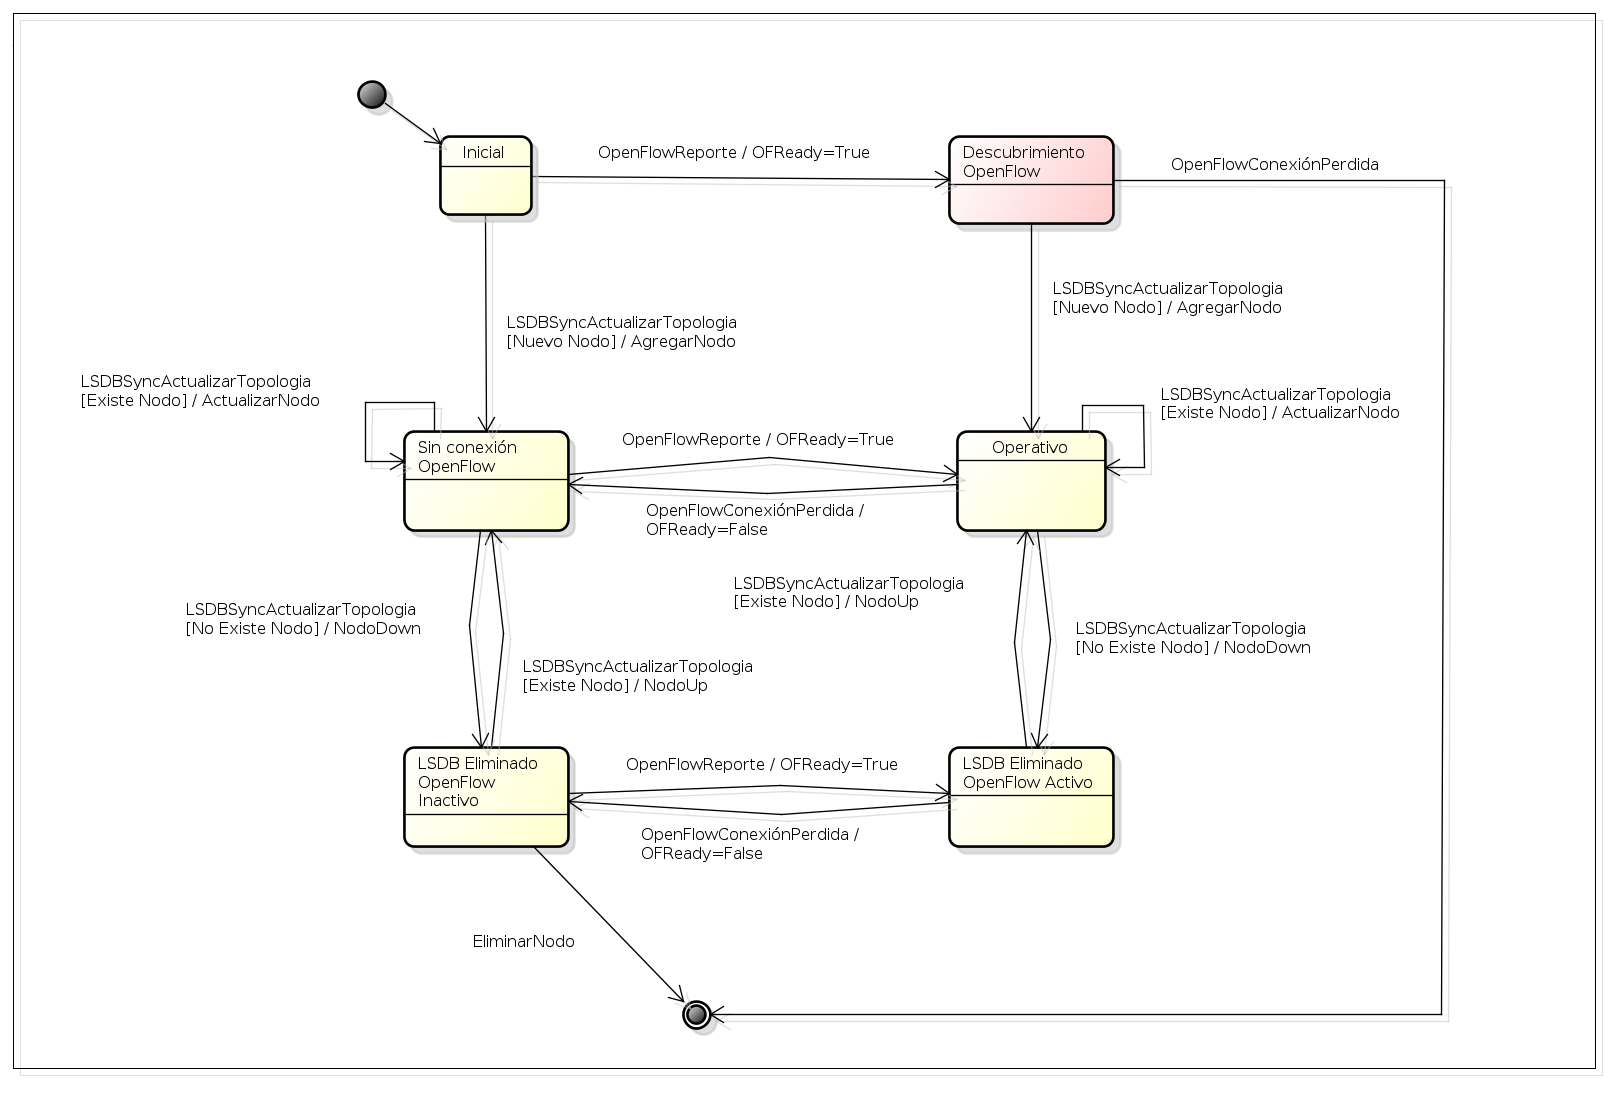
\includegraphics[width=1\textwidth]{CicloVidaNodo2}
\caption[Ciclo de vida de un Nodo]{Ciclo de vida de un Nodo}
\label{fig:CicloVidaNodo}
\end{figure}
  
Como se muestra en la figura\ref{fig:CicloVidaNodo}, descartando el pseudo-estado inicial se identifican cinco estados diferentes para un Nodo: \textit{Descubrimiento OpenFlow}, \textit{Sin Conexión OpenFlow}, \textit{Operativo}, \textit{LSDB Eliminado OpenFlow Inactivo} y \textit{LSDB Eliminado OpenFlow Activo}. El significado de cada uno de estos as\'i como las transiciones posibles se explican a continuación:

\begin{itemize}
\item \textit{Descubrimiento OpenFlow:} Cuando un switch se reporta mediante el canal OpenFlow por primera vez con RAUFlow, se guarda informaci\'on del mismo entre la cual se encuentra la instancia de la clase Datapath en la implementaci\'on de Ryu (esta instancia es utilizada posteriormente para interactuar con el dispositivo). Si el switch OpenFlow no se encuentra instanciado en el Sistema como Nodo, la informaci\'on recibida se almacena en una lista auxiliar de nodos. Como decisión de diseño no se crea una instancia de Nodo como tal a\'un, instanci\'andose solamente cuando se advierte la presencia de \'este en la Link State Database (LSDB).

%Esto se corresponde con una decisión de diseño, en la cual se busca reconocer a un Nodo tanto para las funcionalidades de la interfaz gr\'afica de RAUFlow como para el algoritmo de ruteo, solamente cuando se advierte la existencia del mismo en la inforamci\'on de la LSDB. 

De este estado existen dos transiciones posibles. En primer lugar el switch puede dejar de reportarse con el controlador en cuyo caso es eliminado de la lista temporal de nodos y en segundo lugar la componente LSDBSync puede enviar una actualizaci\'on de la topolog\'ia, en donde se incluye el nodo en cuestión. En este caso se instancia un objeto Nodo con toda la informaci\'on provista por la LSDB, datapath de OpenFlow y la informaci\'on adicional obtenida con el agente SNMP. Luego el Nodo cambia al estado \textit{Operativo}.

Vale la pena destacar que en caso de no poder obtener la informaci\'on adicional con el agente SNMP, el Nodo no es instanciado y se mantiene en el estado actual.

\item \textit{Operativo:}

Este estado es utilizado para representar a aquellos nodos que por un lado se encuentran en la LSDB y fueron rectificados o instanciados en la \'ultima actualizaci\'on de la topolog\'ia, y por otro se encuentran report\'andose mediante el protocolo OpenFlow.

En este estado el nodo es mostrado por la interfaz gr\'afica de RAUFlow y se tiene acceso a todas las características del mismo, tanto del modelo de datos como las que son accesibles a trav\'es del datapath OpenFlow. Adem\'as es considerado para el c\'alculo de las mejores rutas y puede ser utilizado como nodo de ingreso o egreso en la definici\'on de servicios.

En pocas palabras es un nodo completamente funcional a los efectos de la implementaci\'on de RAUFlow.

Desde este estado se tienen tres transiciones posibles. Una primera posibilidad es que se produzca una actualización de la LSDB (evento LSDBSyncActualizarTopologia) y que en la topolog\'ia recibida se encuentre el Nodo en cuesti\'on. En este caso solamente se actualiza la informaci\'on asociada al nodo (acción ActualizarNodo), entre la cual se incluye la actualización de las Interfaces y Links, quedando en el estado actual. Una segunda posibilidad es que el switch asociado deje de reportarse por el canal OpenFlow (evento OpenFlowConexiónPerdida) en cuyo caso se modifica el atributo \textbf{of\_ready} del Nodo asignando el valor False y se cambia al estado \textit{Sin Conexión OpenFlow}. Por \'ultimo una tercera posibilidad es que se produzca una actualizaci\'on de la LSDB (evento LSDBSyncActualizarTopologia) y que el Nodo no este en la topolog\'ia recibida. En este caso se deshabilita el Nodo (NodoDOWN) asignando el valor DOWN al atributo \textbf{state} y se cambia al estado \textit{LSDB Eliminado OpenFlow Activo}.

\item \textit{LSDB Eliminado OpenFlow Activo:} Este estado contempla a un Nodo que no se encontraba en la LSDB recibida en la \'ultima actualizaci\'on topol\'ogica pero que a\'un se reportan por el canal de comunicaci\'on OpenFlow.

Desde este estado se tienen solamente dos transiciones posibles. Una primera posibilidad es que se produzca nuevamente una actualización de la topolog\'ia 
 (LSDBSyncActualizarTopologia) y que el nodo se encuentre dentro de la información recibida. En este caso se actualiza el atributo \textbf{state} del nodo con el valor UP y se cambia al estado \textit{Operativo}. Una segunda posibilidad es que el nodo deje de reportarse por el canal OpenFlow (OpenFlowConexiónPerdida) en cuyo caso se actualiza el valor del atributo \textbf{of\_ready} al valor False y se cambia al estado \textit{LSDB Eliminado OpenFlow Inactivo}.

\item \textit{Sin Conexión OpenFlow:} Este estado contempla a un Nodo que fue creado o rectificado en la \'ultima actualización de la LSDB pero que no se ha reportado por el canal OpenFlow, ya sea porque nunca lo hizo o porque dej\'o de hacerlo. En este estado el Nodo es mostrado a trav\'es de la interfaz gr\'afica de RAUFlow pero no es considerado ni para el el c\'alculo de mejores caminos ni para la creaci\'on de nuevos servicios como nodo de ingreso o egreso. Adem\'as la informaci\'on asociada al datapath de OpenFlow como las tabla de flujos y estad\'isticas tampoco son accesibles.

De este estado existen tres transiciones posibles. Por un lado el nodo puede estar presente en la LSDB al producirse una actualizaci\'on de la topolog\'ia\\ (LSDBSyncActualizarTopologia), actualizándose la informaci\'on del nodo \\ (ActualizarNodo) y manteniéndose en el mismo estado. Por otro lado tambi\'en al producirse una actualizaci\'on de la topolog\'ia, el nodo puede no estar en la LSDB, en cuyo caso se actualiza el atributo \textbf{state} al valor DOWN y se cambia al estado \textit{LSDB Eliminado OpenFlow Inactivo}. Finalmente el switch puede empezar a reportarse por el canal OpenFlow (OpenFlowReport) en cuyo caso se actualiza el valor del atributo \textbf{of\_ready} a True y se cambia al estado \textit{Operativo}.  

\item \textit{LSDB Eliminado OpenFlow Inactivo:} Este estado modela a un Nodo que nunca se report\'o o dej\'o de reportarse por el canal OpenFlow, y que a su vez no se encuentra dentro de la LSDB en la \'ultima actualizaci\'on topol\'ogica realizada. De este estado existen tres transiciones posibles.

Una primera alternativa es que el switch en cuesti\'on se reporte con la aplicaci\'on \\  
 (OpenFlowReporte), en cuyo caso se actualiza el valor del atributo \textbf{of\_ready} a True y se cambia el estado a \textit{LSDB Eliminado OpenFlow Activo}. Una segunda alternativa es que se produzca una actualizaci\'on de la topolog\'ia y el Nodo se encuentre dentro de la LSDB, en cuyo caso se cambia el valor del atributo \textbf{state} a UP y se cambia al estado \textit{Sin conexión OpenFlow}. Finalmente una tercera alternativa es que el nodo  sea eliminado del sistema. Si bien esta funcionalidad no se encuentra actualmente implementada, la idea es que un Nodo para el cual no se ha recibido reportes por el canal OpenFlow luego de un tiempo determinado, y que tampoco aparece en la LSDB tras una actualizaci\'on, pueda ser eliminado del sistema, eventualmente tras la intervenci\'on de un usuario administrador.
  
\end{itemize}

El ciclo de vida de una Interfaz o un Link puede ser explicado de forma an\'aloga con una m\'aquina de estados similar, teniendo presente las relaciones existentes entre las tres clases, Nodos, Interfaces y Links.

\subsection{QoS en RAUFlow}
Por razones de tiempo no se implementaron en RAUFlow funcionalidades de QoS como balanceo de carga y asignaci\'on de prioridades por tipo de tr\'afico. Sin embargo, a continuaci\'on se describen las alternativas a explorar en caso de seguir con el desarrollo de esta aplicaci\'on.

Dentro de las funcionalidades de calidad de servicio (QoS) que se podrían implementar en RAUFlow interesan dos principalmente: (1) la capacidad para construir caminos alternativos para un servicio y  de esta forma hacer balanceo de carga entre todos los LSPs constru\'idos y (2) asignar prioridades por servicio para el procesamiento de tr\'afico en cada uno de los nodos de la red.

Para la construcci\'on de caminos alternativos para un mismo servicio existen dos soluciones: (1) una soluci\'on simple la cual permite a un administrador definir manualmente caminos y (2) una soluci\'on m\'as compleja en la que se mejora el algoritmo de ruteo centralizado para implementar un CSPF que permita calcular diferentes caminos para un mismo par nodo-interfaz de ingreso y egreso, en funci\'on del ajuste de diferentes par\'ametros de QoS (ancho de banda por ejemplo). 

Para implementar (1) en el prototipo es necesario modificar levemente la implementaci\'on de la clase Servicio para distinguir entre los servicios en que el LSP se calcula con el algoritmo de ruteo y los que se definen de forma manual, a la vez que es necesario extender la interfaz gr\'afica para implementar este nuevo caso de uso. 

Para implementar (2) se requiere de un tiempo de desarrollo considerablemente mayor que en la alternativa (1) puesto que es necesario modificar el algoritmo de ruteo e implementar un CSPF.\\ 

Asumiendo que se soportan m\'ultiples caminos para un mismo servicio, puede implementarse balanceo de carga de dos formas: (1) “partir” la definici\'on de un servicio de VPN en varios subservicios diferenciando por el tipo de tr\'afico mediante el cabezal OpenFlow y as\'i hacer balanceo de carga por ejemplo por tipo de aplicaci\'on, (2) implementar balanceo de carga basándose en las estadísticas de los flujos OpenFlow y así balancear din\'amicamente el tr\'afico de un servicio de VPN entre diferentes caminos.

Para implementar (1) solo es necesario que RAUFlow implemente alguno de los mecanismos mencionados para la definición de múltiples caminos para un servicio. 

Por otro lado para implementar (2) se puede utilizar el concepto de “Meters” o m\'etricas de OpenFlow que permiten analizar la cantidad de paquetes procesados por un mismo flujo y en funci\'on de esto aplicar una acci\'on o conjunto de acciones. Sin embargo Open vSwitch no implementa esta característica del protocolo, por lo que no es posible implementarlo en RAUFlow; de hecho Open vSwitch ofrece otras funcionalidades de QoS que delega al kernel de Linux en vez de implementar los mecanismos contemplados por el protocolo OpenFlow. 

Dentro de las funcionalidades de QoS que implementa Open vSwitch se encuentran la definici\'on de “colas” a las que se les puede definir tasas de transferencia mínima y máxima. Mediante esta funcionalidad es posible implementar prioridades por tipo de tr\'afico y asi por servicio, aunque como es una implementaci\'on propia de la herramienta no puede ser manipulada din\'amicamente desde el controlador mediante el protocolo OpenFlow.\\

De esta forma queda explicada la implementaci\'on de la aplicaci\'on de gesti\'on RAUFlow, el diseño de  los nodos que formar\'an parte de la red prototipo (RAU-Switch) y el funcionamiento general del prototipo en su conjunto. El siguiente cap\'itulo est\'a destinado al diseño y construcción de un laboratorio de pruebas, para la validaci\'on de las componentes desarrolladas y la implementaci\'on de algunos casos de uso representativos. 



